\documentclass{article}
\usepackage{graphicx}
\begin{document}
\setcounter{section}{3}
\section{Recurrence}
\subsection*{Substitution Example}
\begin{eqnarray}
T(n) & = & cn \\
T(n+1) & = & = c(n + 1) \\
& = & T(n) + c \\
& = & cn + c \\
& = & c(n + 1)
\end{eqnarray}

\subsection*{Recursion Tree}
$2T(n/2) + n^2$.

\noindent\makebox[\textwidth]{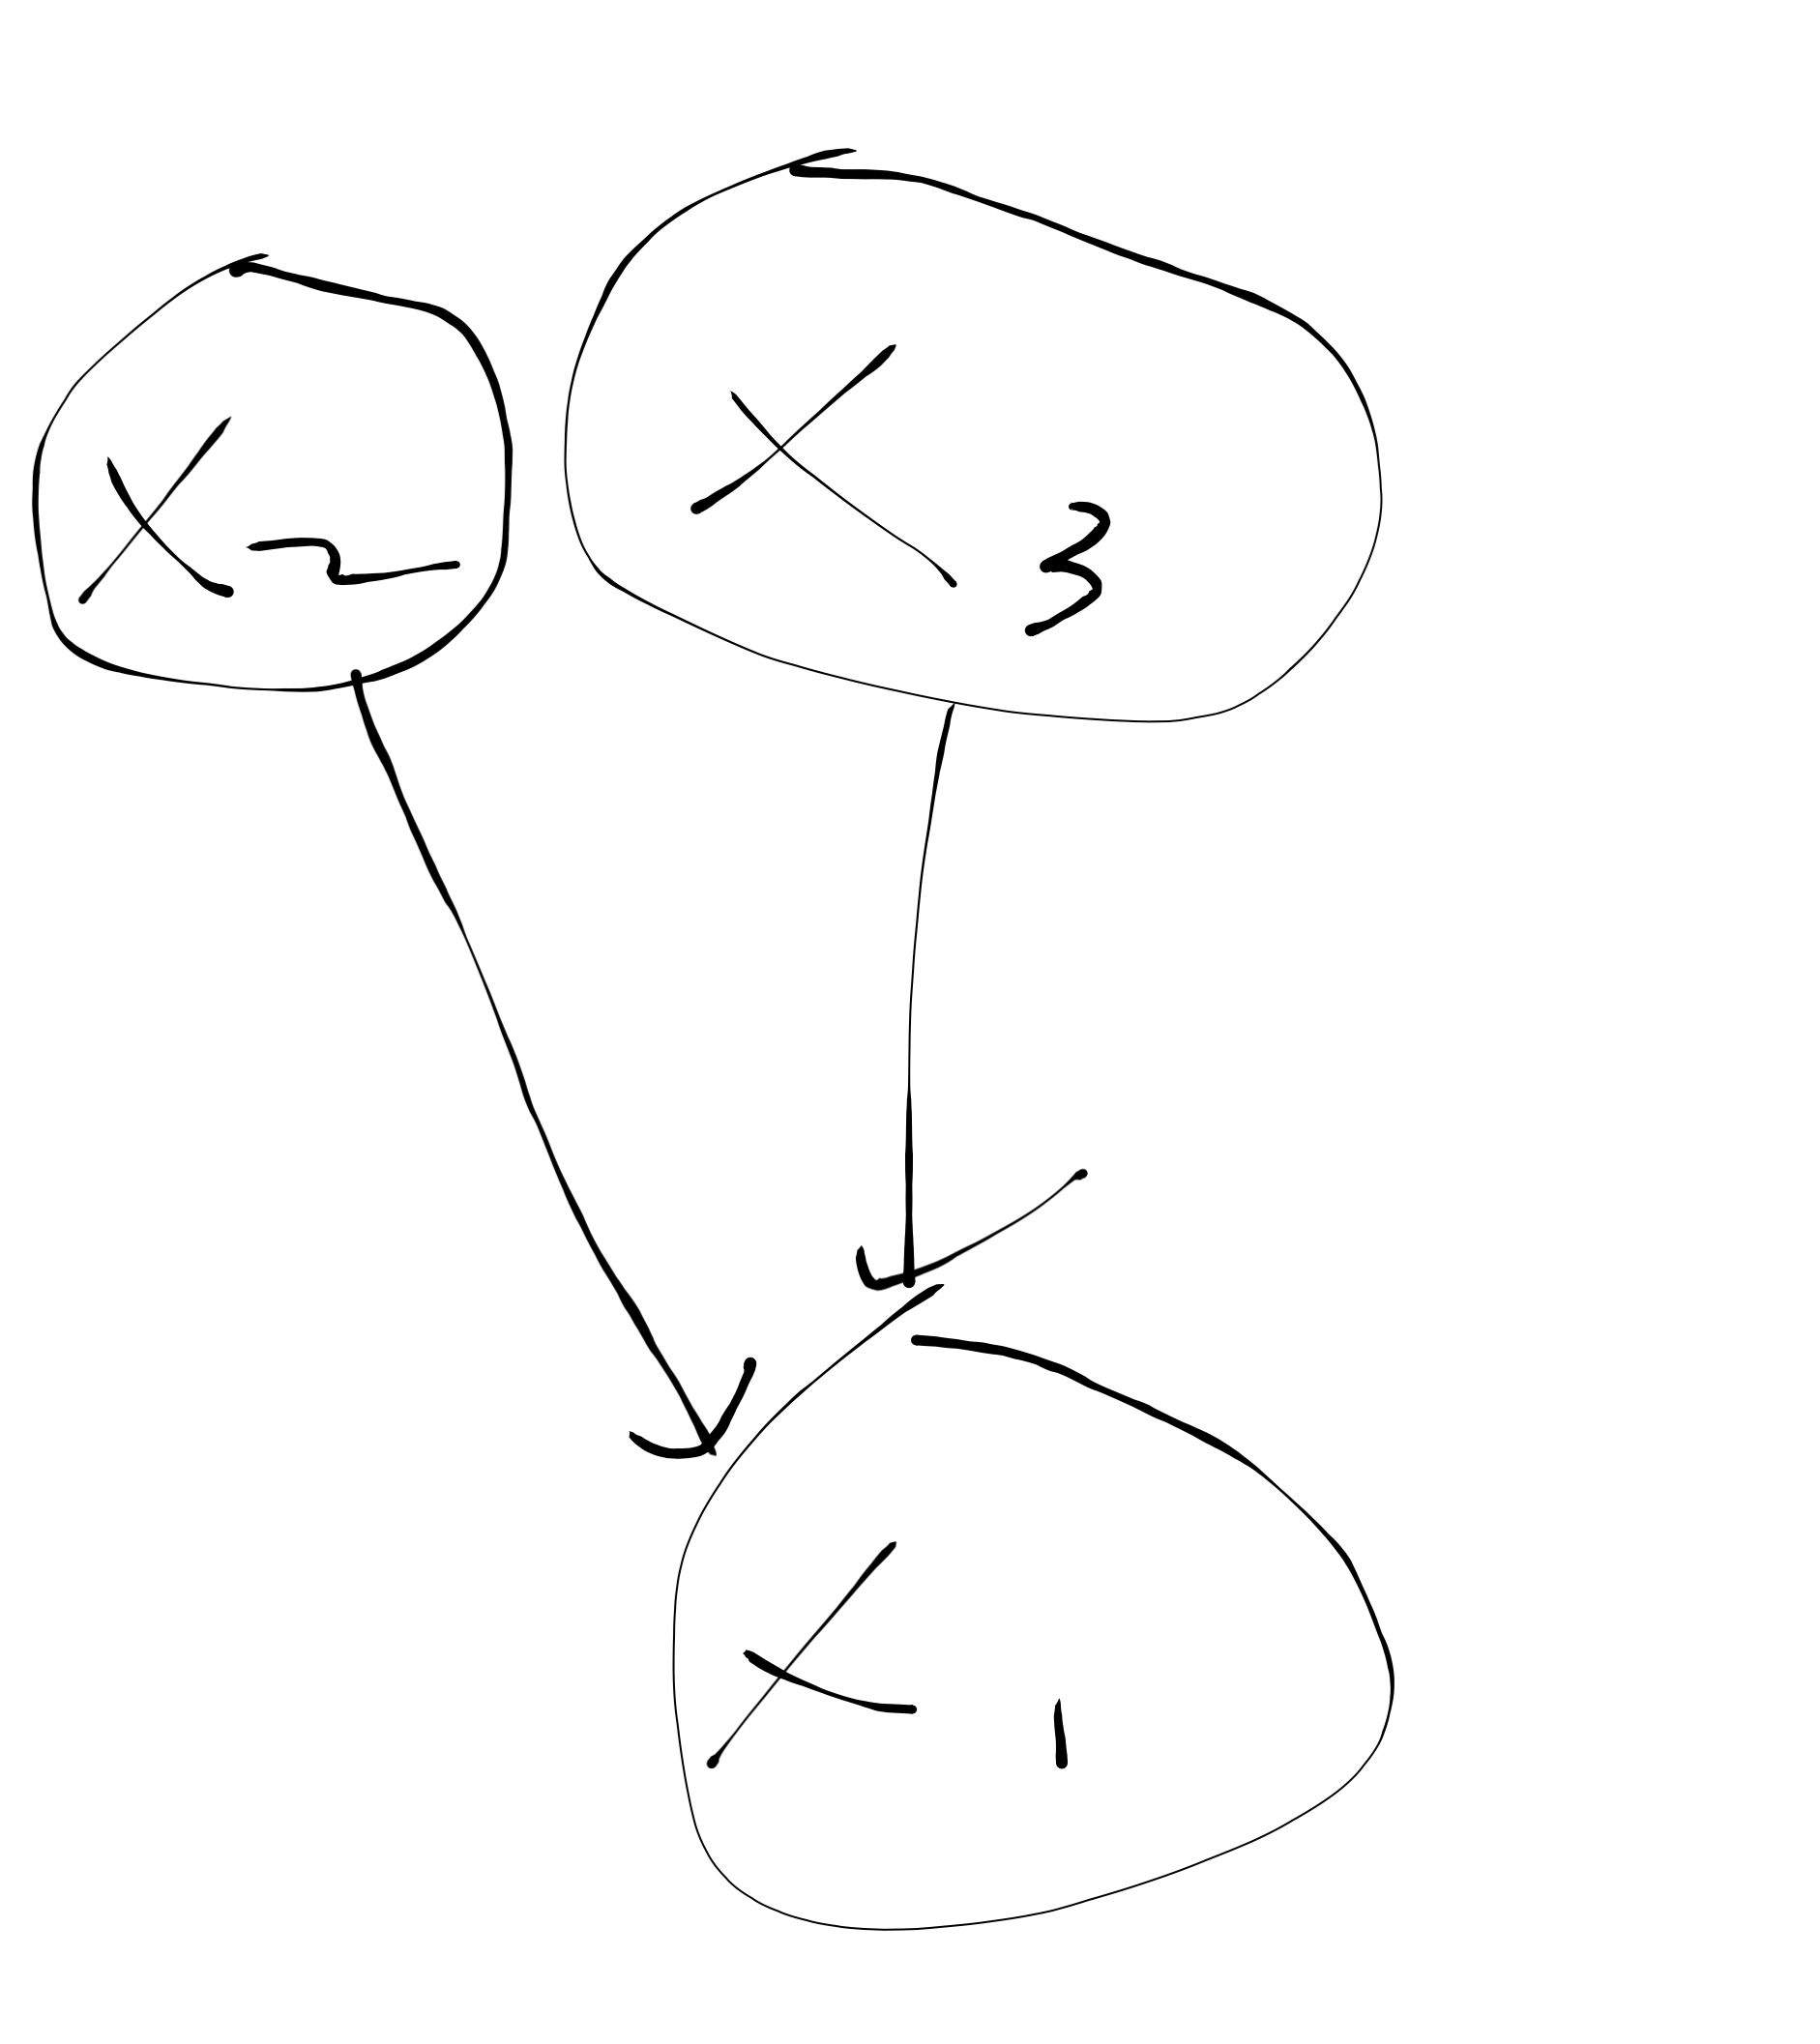
\includegraphics[width=\paperwidth]{1}}

\subsubsection*{Master Theorem}
Check given $T(n)$ is the form of $aT(n/b) + f(n)$

\begin{equation}
T(n) = 8 T (n/2) + n^2
\end{equation}

$a = 8, b = 2, f(n) = n^2$. Prove $f(n) \in O(n^{log _2 a- \epsilon)} = O(n^{3- \epsilon}) = O(n^{3 - 1}) = O(n^2)$. $T(n) = \Theta (n^{log _b a}) = \Theta (n^3)$
\end{document}